%Made By Thomas Debelle
\documentclass{report}
\usepackage[a4paper, total={6in, 9in}]{geometry}
\usepackage[utf8]{inputenc}
\usepackage[francais]{babel}
\usepackage{graphicx}
\usepackage{graphics}
\usepackage[T1]{fontenc}
\usepackage{amsmath}
\usepackage{hyperref}
\usepackage{amssymb}
\usepackage{listings}
\usepackage{wrapfig}
\usepackage{xcolor}
\usepackage{array}
\usepackage{float}
\usepackage{amsfonts}
\usepackage{fancyhdr}
\usepackage{titlesec}
\usepackage{xparse}

\hypersetup{
    colorlinks=true,
    linkcolor=black,
    filecolor=magenta,
    urlcolor=cyan,
    pdftitle={Overleaf Example},
    pdfpagemode=FullScreen,
    }
\begin{document}


\begin{titlepage}
    \begin{figure}
        
\includegraphics[height = 2cm]{UCL_Logo.png}
        \label{fig:my_label}
    \end{figure}

    \hspace*{100cm}
    \centering
    \vspace*{7cm}

    {\Huge \textbf{Résumé de LINFO1104}}\\
    \vspace*{0.25cm}
    compilation du \today\\
    \vspace*{0.25cm}
    \Large{Thomas Debelle}\\

    \vspace*{9.5cm}
    {\Large Juin 2023}
\end{titlepage}


\tableofcontents
\newpage

\section*{Préface}

Bonjour à toi !\\

Cette synthèse recueille toutes les informations importantes données au cours, pendant les séances de tp et est amélioré grâce au note du Syllabus. Elle ne remplace pas le cours donc écoutez bien les conseils et potentielles astuces que les professeurs peuvent vous donner. Notre synthèse est plus une aide qui on l'espère vous sera à toutes et tous utiles.\\

Elle a été réalisée par toutes les personnes que tu vois mentionné. Si jamais cette synthèse a une faute, manque de précision, typo ou n'est pas à jour par rapport à la matière actuelle ou bien que tu veux simplement contribuer en y apportant ta connaissance ? Rien de plus simple ! Améliore la en te rendant \href{http://www.github.com/Tfloow/Q4_EPL}{ici} où tu trouveras toutes les infos pour mettre ce document à jour. (\textit{en plus tu auras ton nom en gros ici et sur la page du github})\\

Nous espérons que cette synthèse te sera utile d'une quelconque manière ! Bonne lecture et bonne étude.


\chapter{Introduction}
\section{Les Paradigmes}
Une paradigme, est une façon d'approcher et apporter une solution à un problème. De ce fait, chaque langage de programmation utilise 1 voir 2 paradigmes. Ce cours couvrat 5 paradigmes cruciaux qui sont:
\begin{enumerate}
\item "Functionnal Programming"
\item "Object Oriented Programming"
\item "Functional DataFlow Programming"
\item "Actor DataFlow Programming or Multi-Agent"
\item "Active Objects"
\end{enumerate}

Et pour découvrir ces paradigmes, nous utiliserons les langages de programmations \href{https://fr.wikipedia.org/wiki/Oz_(langage)}{"Oz"} qui est un langage de recherche multi paradigme ainsi que \href{https://fr.wikipedia.org/wiki/Erlang_(langage)}{"Erlang"}.

\chapter{Les différents Paradigmes}
Comme mentionner plus haut, on rencontrera 5 paradigmes dont voici le premier.
\section{Functional Programming}
Avec ce paradigme, on impose qu'une variable peut être nommé qu'une seule fois ! Donc: \quad X = 10 mais on ne peut pas plus loin dire X = 9. X est déjà attribué. On peut penser que cela risque d'être handicapant alors qu'en réalité, cela rend notre code plus simple à débugger. De plus, nombreux sont les langages et microservices utilisés qui implémentent la programmation fonctionnelle.
Formellement, quand on déclare une variable et qu'on l'assigne à une valeur ceci se passe.
\begin{wrapfigure}{r}{.4\textwidth}
	\centering
    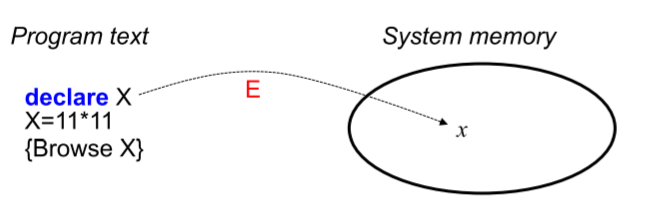
\includegraphics[width=.5\textwidth]{img/declVar.png}
    \caption{Déclaration d'une variable}
\end{wrapfigure}
Une chose importante à noter est que cette façon de programmer peut être réalisé dans n'importe quel langage de programmation. On peut également redéclarer un identificateur. C'est-à-dire écrire "X = 42" et plus loin en ayant redéclarer une variable "X = 11" car ces deux déclarations pointent à deux éléments totalement différents dans la mémoire.\\

Un "Scope" ou portée est une propriété centrale en programmation. En effet, c'est le scope qui nous permet d'avoir différente valeur pour des variables qui ont le même nom. Naturellement, elle ne représente pas la même chose car elle diffère de leur scope. On peut déterminer le scope d'une variable sans même exécuter le code. Il nous suffit d'analyser le code qui comprend un "\textcolor{red}{lexical scoping}" ou un "\textcolor{red}{static scoping}".
\begin{figure}[H]
\centering
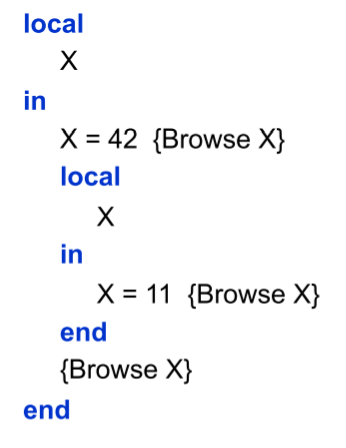
\includegraphics[width=3cm]{img/scope.png}
\caption{Exemple de code avec des scope différents}
\end{figure}
\section{Conseils pour la syntaxe d'Oz}

\end{document}
